\documentclass[a4paper,11pt]{article}
% Packages de base
\usepackage[utf8]{inputenc}
\usepackage[french]{babel}
\usepackage[T1]{fontenc}

% Packages de maths
\usepackage{amsmath}
\usepackage{amssymb}
\usepackage{mathrsfs}

% Mise en page
\usepackage[top=2.5cm, bottom=2.5cm, left=2.5cm, right=2.5cm]{geometry}
\usepackage{hyperref}
\usepackage{xcolor}
\hypersetup{
    colorlinks,
    linkcolor={red!50!black},
    citecolor={blue!50!black},
    urlcolor={blue!80!black}
}
\usepackage{graphicx}


\title{Travaux Pratiques Hadoop}
\author{Grégoire MASSOT - \href{http://www.gregoire-massot.com}{gregoire-massot.com}}
\date{14 Novembre 2015. MàJ le 1 Avril 2016}

\begin{document}

\maketitle

Voici un compte-rendu des TPs Hadoop réalisés lors du cours Big Data en 3ème année à l'École des Mines, entre Septembre et Novembre 2015.\\
Ces TPs ont été réalisés sous Windows avec la machine virtuelle \href{http://www.cloudera.com/downloads/quickstart_vms/5-5.html}{Cloudera CDH 5.5}.

\begin{figure}[ht!]
\centering
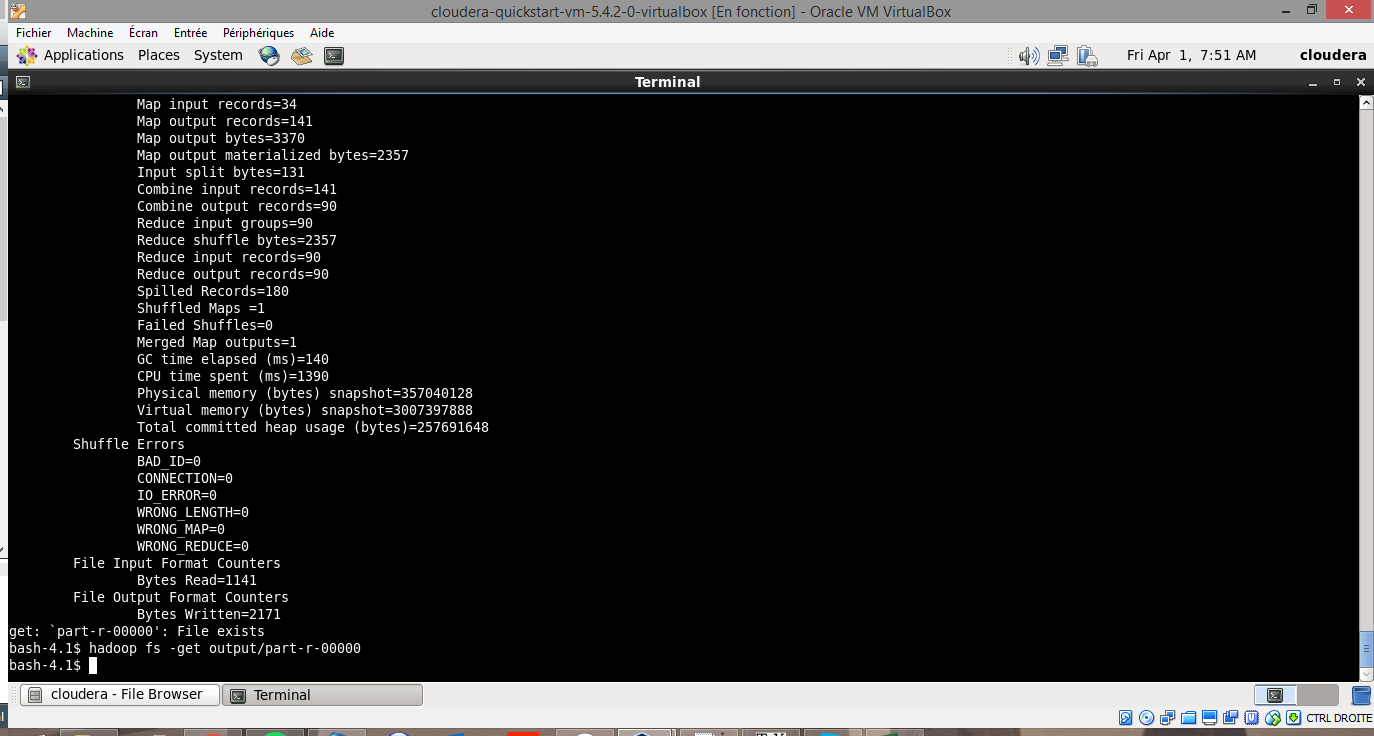
\includegraphics[width=10cm]{Screenshot.png}
\caption{Screenshot de la VM CDH5.5 de Cloudera \label{overflow}}
\end{figure}

\section{initialize.sh et launch.sh}

Ce sont les scripts qui permettent respectivement d'automatiser les tâches d'initialisation de la machine virtuelle et d'exécution du programme. Plus de détails dans les commentaires.

\section{tinygraph.txt}

Le fichier d'entrée \texttt{tinygraph.txt} est un graphe de pages web. Chaque ligne correspond à une page web. Pour chaque ligne $i$ :
\begin{itemize}
\item  Le premier nombre est le numéro associé à la page web $i$
\item  Le second nombre est le PageRank initial de la page $i$. Il est égal à $\frac{1}{N}$ où $N$ est le nombre de pages web contenues dans le graphe
\item Les nombres suivants sont les numéros associés aux pages vers lesquels pointent les liens hypertextes de la page $i$
\end{itemize}


\section{pageRank.java}

C'est le programme qui va calculer les Page Rank des pages contenues dans \texttt{tinygraph.txt}.

\begin{itemize}
\item \textbf{Map} : Pour chaque ligne $i$ on liste les liens sortants $j$ et on produit les couples clé-valeur (page web $j$, $\frac{1}{N_{i}}$) avec $N_{i}$ le nombre de liens sortants de la page $i$.
\item \textbf{Reduce} : pour chaque paire clé-valeur, on sort somme les valeurs et on sort (page web $j$, somme valeurs associées à la clé $j$)
\end{itemize}

\section{part-r-000000}

C'est le fichier de sortie fourni par notre cluster Hadoop. Chaque ligne représente une page web. Pour chaque ligne $i$
\begin{itemize}
\item Le premier nombre correspond au numéro de la page web $i$
\item Le second nombre est le PageRank de la page après calcul.
\end{itemize}

\end{document}